\begin{figure}
    \centering
    \begin{subfigure}{0.3\linewidth}
        \centering
        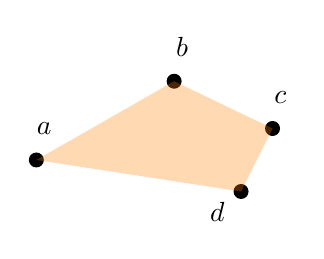
\begin{tikzpicture}
            \node[draw, circle, black, fill=black, inner sep=0pt, minimum size=5pt, label={[xshift=0.1cm, yshift=0.1cm]$a$}] (a) at (0,0) {};
            \node[draw, circle, black, fill=black, inner sep=0pt, minimum size=5pt, label={[xshift=0.1cm, yshift=0.1cm]$b$}] (b) at (1.75,1) {};
            \node[draw, circle, black, fill=black, inner sep=0pt, minimum size=5pt, label={[xshift=0.1cm, yshift=0.1cm]$c$}] (c) at (3,0.4) {};
            \node[draw, circle, black, fill=black, inner sep=0pt, minimum size=5pt, label={[xshift=-0.3cm, yshift=-0.6cm]$d$}] (d) at (2.6,-0.4) {};
            \coordinate (a) at (0,0);
            \coordinate (b) at (1.75,1);
            \coordinate (c) at (3,0.4);
            \coordinate (d) at (2.6,-0.4);
            \fill[orange, opacity=0.3] (a) -- (b) -- (c) -- (d) -- (a) -- cycle;
        \end{tikzpicture}
        \caption{The signature induced by $\sigma$ is $\texttt{-\,-\,-\,-}$.}
    \end{subfigure}
    \begin{subfigure}{0.3\linewidth}
        \centering
        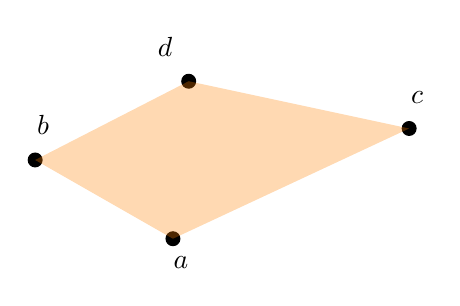
\begin{tikzpicture}
            \node[draw, circle, black, fill=black, inner sep=0pt, minimum size=5pt, label={[xshift=0.1cm, yshift=-0.6cm]$a$}] (a) at (0,0) {};
            \node[draw, circle, black, fill=black, inner sep=0pt, minimum size=5pt, label={[xshift=0.1cm, yshift=0.1cm]$b$}] (b) at (-1.75,1) {};
            \node[draw, circle, black, fill=black, inner sep=0pt, minimum size=5pt, label={[xshift=0.1cm, yshift=0.1cm]$c$}] (c) at (3,1.4) {};
            \node[draw, circle, black, fill=black, inner sep=0pt, minimum size=5pt, label={[xshift=-0.3cm, yshift=0.1cm]$d$}] (d) at (0.2,2) {};
            \coordinate (a) at (0,0);
            \coordinate (b) at (-1.75,1);
            \coordinate (c) at (3,1.4);
            \coordinate (d) at (0.2,2);
            \fill[orange, opacity=0.3] (b) -- (d) -- (c) -- (a) -- (b) -- cycle;
        \end{tikzpicture}
        \caption{The signature induced by $\sigma$ is $\texttt{-\,-\,+\,-}$.}
    \end{subfigure}
    \begin{subfigure}{0.3\linewidth}
        \centering
        
\begin{tikzpicture}
            \node[draw, circle, black, fill=black, inner sep=0pt, minimum size=5pt] (p) at (0,0) {};
        \end{tikzpicture}
    \end{subfigure}
  \caption{Illustration of the notion of $\sigma$-equivalence.}\label{fig:sigma-equiv}
  \end{figure}